\documentclass[12pt]{article}
\usepackage{amsmath}
%\usepackage{longtable}
\usepackage{graphicx,psfrag,epsf}
\usepackage{enumerate}
\usepackage{natbib}
\usepackage{tcolorbox}
\usepackage{fontawesome}
\usepackage{booktabs}
\usepackage{float}
\usepackage{url} % not crucial - just used below for the URL
\providecommand{\tightlist}{%
  \setlength{\itemsep}{0pt}\setlength{\parskip}{0pt}}

%\pdfminorversion=4
% NOTE: To produce blinded version, replace "0" with "1" below.
\newcommand{\blind}{1}

% need this for pandoc %
\newlength{\cslhangindent}
\setlength{\cslhangindent}{1.5em}
\newlength{\csllabelwidth}
\setlength{\csllabelwidth}{3em}
\newenvironment{CSLReferences}[3] % #1 hanging-ident, #2 entry spacing
 {% don't indent paragraphs
  \setlength{\parindent}{0pt}
  % turn on hanging indent if param 1 is 1
  \ifodd #1 \everypar{\setlength{\hangindent}{\cslhangindent}}\ignorespaces\fi
  % set entry spacing
  \ifnum #2 > 0
  \setlength{\parskip}{#2\baselineskip}
  \fi
 }%
 {}
\usepackage{calc} % for \widthof, \maxof
\newcommand{\CSLBlock}[1]{#1\hfill\break}
\newcommand{\CSLLeftMargin}[1]{\parbox[t]{\maxof{\widthof{#1}}{\csllabelwidth}}{#1}}
\newcommand{\CSLRightInline}[1]{\parbox[t]{\linewidth}{#1}}
\newcommand{\CSLIndent}[1]{\hspace{\cslhangindent}#1}


% DON'T change margins - should be 1 inch all around.
\addtolength{\oddsidemargin}{-.5in}%
\addtolength{\evensidemargin}{-.5in}%
\addtolength{\textwidth}{1in}%
\addtolength{\textheight}{1.3in}%
\addtolength{\topmargin}{-.8in}%

%-------------------------------------------------------------------
% R MARKDOWN
%-------------------------------------------------------------------
\IfFileExists{bookmark.sty}{\usepackage{bookmark}}{\usepackage{hyperref}}

\def\spacingset#1{\renewcommand{\baselinestretch}%
{#1}\small\normalsize} \spacingset{1}


\begin{document}

%\bibliographystyle{natbib}

\def\spacingset#1{\renewcommand{\baselinestretch}%
{#1}\small\normalsize} \spacingset{1}


%%%%%%%%%%%%%%%%%%%%%%%%%%%%%%%%%%%%%%%%%%%%%%%%%%%%%%%%%%%%%%%%%%%%%%%%%%%%%%

\if0\blind
{
  \title{\bf The Journey from Wild to Textbook Data: A Case Study from the National Longitudinal Survey of Youth}
  \author{
            Dewi Amaliah\thanks{Corresponding author, \href{mailto:dlamaleeah@gmail.com}{\nolinkurl{dlamaleeah@gmail.com}}}\\
      Dept of Econometrics and Business Statistics, Monash University, \\
            Dianne Cook\\
      Dept of Econometrics and Business Statistics, Monash University, \\
            Emi Tanaka\\
      Dept of Econometrics and Business Statistics, Monash University, \\
            Kate Hyde\\
      Dept of Econometrics and Business Statistics, Monash University, \\
            Nicholas Tierney\\
      , Telethon Kids Institute, }
        \maketitle
} \fi

\if1\blind
{
  \bigskip
  \bigskip
  \bigskip
  \begin{center}
    {\LARGE\bf The Journey from Wild to Textbook Data: A Case Study from the National Longitudinal Survey of Youth}
\end{center}
  \medskip
} \fi

\bigskip
\begin{abstract}
The National Longitudinal Survey of Youth (NLSY79) is a prominent open data source that has been important for educational purposes and multidisciplinary research on longitudinal data. Subsets of this data can be found in numerous textbooks and research articles. However, the steps and decisions taken to get from the raw data to the textbook data are never clearly articulated. This article describes our journey when trying to re-create a textbook example data set from the original database, with the goal being to refresh the textbook data more regularly. Thus, this paper demonstrates the process -- extracting, tidying, cleaning, and exploring with documentation -- to make refreshed data available for education or research. Three new data sets and the code to produce them are provided in an accompanying open source R package, called {[}CENSORED{]}. As a result of this process, some recommendations are also made for the NLSY79 curators for incorporating data quality checks and providing more convenient samples of the data to potential users.
\end{abstract}

\noindent%
{\it Keywords:}  Data cleaning; Data tidying; Reproducible workflow; Longitudinal data; NLSY79; Initial data analysis;
\vfill

\newpage
\spacingset{1.45} % DON'T change the spacing!

\hypertarget{intro}{%
\section{Introduction}\label{intro}}

Statistics and data science education relies on cleaned and simplified data, suitably called textbook data, for clear examples about how to apply different techniques. An example of this, is the wages data made public by Singer and Willett (2003) which can be used to teach generalized linear models, including hierarchical, mixed effects and multilevel. The freely available data records hourly wages of a sample of high school dropouts, from 1979-1994, along with demographic variables including education and race, taken from the National Longitudinal Survey of Youth (NLSY79) (Bureau of Labor Statistics, U.S. Department of Labor 2021).

The story from modeling the data (and as reported by Singer and Willett) is that wages increase with the length of time in the workforce, higher level of education leads to higher wages, and that race makes a difference, on average. An exploratory analysis reveals however that the individual experience varies a great deal from the overall average. Some individuals experience a decline in wages the longer they are in the workforce, and many experience volatility in their wages. The wages data was used to illustrate exploratory longitudinal data analysis in Ozlem Ilk's PhD thesis supervised by author Cook (Ilk 2004), and was further developed into a case study for use in the teaching of exploratory data analysis at Iowa State University.

This textbook data was used as an example in Ilk (2004), and was developed into a case study for use in teaching exploratory data analysis at CENSORED. The story from modeling the data (and as reported by Singer and Willett) is that wages increase with the length of time in the workforce, higher level of education leads to higher wages, and that race makes a difference, on average. An exploratory analysis reveals however that the individual experience varies a great deal from the overall average. Some individuals experience a decline in wages the longer they are in the workforce, and many experience volatility in their wages.

This disparity between the average and the individual is a part of statistics, as a discipline, that is given less attention. It is this disparity which makes this particular data set important as a textbook example. Textbook data sets have longevity if there is a unresolved mystery. The iris data (Andereson 1935) is a prime example. It has withstood the test of time because the three species cannot be perfectly classified, and so it continues to challenge researchers and instructors to do better in the analysis. (A side note: the iris data is best replaced today with the penguins data (Horst, Hill, and Gorman 2020), which has similar qualities, is new and does not suffer from a connection with eugenics (Stodel 2020).) We argue that the wages data is in this class of textbook data, too, because it presents a challenge for longitudinal data analysis: how can we better summarize and explain the individual experience?

For the field of statistics, and data science by association, it is increasingly important to reach the individual. One might describe this as a divergence of purpose, statistics for public policy or statistics for the public. The two are not the same. As the world becomes more electronically connected combating misinformation and mitigating conspiracy theories require that statistics address the individual. For example, with the wages data, even though the message for public policy is that demographic profile is related to different wage patterns on average, the message for the individual is that you are more than your demographic. The majority of people in the study do not have a pattern that is similar to the average. If you have a bad experience, that your wages have declined over time, you are not alone, there are others like you, and more than you think. {[}ET: a related article: \url{https://www.smh.com.au/national/by-the-numbers--the-average-australian-doesnt-exist--not-a-single-one-of-us-is-normal-20150124-12xlh0.html}{]}

As a textbook data set though, it is outdated. The most recent year in the data is 1994, 10 years prior to when Singer and Willett (2003) was published. Teachers of statistics need use contemporary data sets to show how techniques are relevant to today's students. Using tired old textbook data sets can imbue a misconception that the field is not current. The wages data is extracted from NSLY79, one of the best examples of open data, which is constantly being updated. It should be possible to continuously refresh the textbook data from the data repository. This paper describes our (non-glamorous) journey from open (Open Knowledge Foundation 2021) wild data to textbook data.

This paper demonstrates the steps of cleaning data, and documents the process, as recommended by Huebner, Vach, and Cessie (2016). They emphasize that making the data cleaning process accountable and transparent is imperative and essential for the integrity of downstream statistical analyses and model building. Data cleaning can be considered to be a part of what is called ``initial data analysis'' (IDA) (Chatfield 1985). In IDA one would also explore the data, especially to check if the data is consistent with assumptions required for modeling. This is also related to exploratory data analysis (EDA), coined by Tukey (1977) with a focus on learning from data. EDA can be considered to encompass IDA. Dasu and Johnson (2003) say that data cleaning and exploration, without naming it as IDA, is a difficult task and consumes 80\% of the data mining task.

<<<<<<< HEAD
Our process of cleaning builds heavily on the \texttt{tidyverse} approach (Wickham, Averick, et al. 2019). The data is first organized into ``tidy data'' (Wickham 2014) and then further wrangled using the data pipeline and split-apply-combine approach (Wickham 2011). (Tidy data shouldn't be confused with ``tame data'' which Kim, Ismay, and Chunn (2018) coined to refer to textbook data sets suitable for teaching, particularly teaching statistics.) The resulting (tame) data is provided in a new R package called \texttt{[CENSORED]} which includes the code so that the process is reproducible, and could be used to further refresh the data as new records are made available in the NLSY79 database.
=======
Our process of cleaning builds heavily on the \texttt{tidyverse} approach (Wickham et al. 2019). The data is first organized into ``tidy data'' (Wickham 2014) and then further wrangled using the data pipeline and split-apply-combine approach (Wickham 2011). (Tidy data shouldn't be confused with ``tame data'' which Kim, Ismay, and Chunn (2018) coined to refer to textbook data sets suitable for teaching, particularly teaching statistics.) The resulting (tame) data is provided in a new R package called \texttt{[CENSORED]} which includes the code so that the process is reproducible, and could be used to further refresh the data as new records are made available in the NLSY79 database.
>>>>>>> e9174550e6e3a231aa9c7572667f6c47600e0929

This paper is structured in the following way. Section \ref{database} describes the NLSY79 data source. Section \ref{cleaning} presents the steps of cleaning the data, including getting and tidying the data from the NLSY79 and IDA to find and repair anomalies. Our final subset is compared to the old textbook subset in Section \ref{compare}. Finally, Section \ref{summary} summarizes the contribution and makes recommendations for the NLSY79 data curators.

\hypertarget{database}{%
\section{The NLSY79}\label{database}}

Singer and Willett (2003) used the wages and other variables of high school dropouts from the NLSY79 data as an example data set to illustrate longitudinal data modeling of wages on workforce experience, with covariates education and race. This data has been playing an important role in research in various disciplines, including but not limited to economics, sociology, education, public policy, and public health for more than a quarter of the century (Pergamit et al. 2001). In addition, this is considered a carefully designed longitudinal survey with high retention rates, making it suitable for life course research (Pergamit et al. 2001; Cooksey 2017). According to Cooksey (2017), thousands of articles, and hundreds of book chapters and monographs have utilized this data. Moreover, the NLSY79 is considered the most widely used and most important cohort in the survey data (Pergamit et al. 2001).
Our aim is to refresh this textbook data and append it with data from 1994 through to the latest data reported in 2018, a purpose that is consistent with Grimshaw (2015)'s statistics education goal of embracing authentic data experiences. Here, we investigate the process of getting from the raw NLSY79 data to a textbook data set as similar as possible to that provided by Singer and Willett (2003). We should also note that race is a variable in the original data set, and for compatibility it is also provided with the refreshed data, for the \emph{purposes of studying racism, not race} (Fullilove 1998).

\hypertarget{database-1}{%
\subsection{Database}\label{database-1}}

The NLSY79 is a longitudinal survey administered by the U.S Bureau of Labor Statistics that follows the lives of a sample of American youth born between 1957-1964 (Bureau of Labor Statistics, U.S. Department of Labor 2021). The cohort originally included 12,686 respondents aged 14-22 when first interviewed in 1979. It comprised of people sampled because they were Blacks, Hispanics, economically disadvantaged non-Black non-Hispanics, and youth in the military. In 1984 and 1990, two sub-samples were dropped from the interview; the dropped subjects were the 1,079 members of the military sample and 1,643 members who represents economically disadvantage people, but were not Black nor Hispanics, respectively. These subsamples were dropped because they are not eligible anymore for interview (Bureau of Labor Statistics, U.S. Department of Labor 2021). Hence, 9,964 respondents remain in the eligible samples. The surveys were conducted annually from 1979 to 1994 and biennially thereafter. Data are currently available from Round 1 (1979 survey year) to Round 28 (2018 survey year).

Although the main focus area of the NLSY is labor and employment, the NLSY also covers several other topics, including education, training, achievement, household, geography, dating, marriage, cohabitation, sexual activity, pregnancy, fertility, children, income, assets, health, attitudes and expectations, crime, and substance use.

There are two ways to conduct the interview of the NLSY79, which are face-to-face or by telephone interviews. In recent survey years, more than 90 percent of respondents were interviewed by telephone (Cooksey 2017).

\hypertarget{target}{%
\subsection{Target data}\label{target}}

The NLSY79 data used in Singer and Willett (2003) contains the longitudinal measurements on yearly mean hourly wages with years of workforce experience, and demographic variables education and race, from 1979 through to 1994. In addition, the cohort is restricted to male high-school dropouts who first participated in the study at age 14-17 years.
Thus the target data set is to collect the same variables for the extended time frame of 1994 through to 2018, the most recent year reported.

\hypertarget{cleaning}{%
\section{Data cleaning}\label{cleaning}}

van der Loo and de Jonge (2018) describe the notion of a ``statistical value chain'' where the production stages of the data cleaning process are earmarked as raw data (data as arrived to the desk of an analyst), input data (data organised with correct type and identified variables) and valid data (data that faithfully represent the variables). In this section, we outline the steps to download the raw data (Section \ref{getdata}) and then tidy the raw data into input data, specifically for the demographic variables (Section \ref{tidydemog}) and the employment variables (Section \ref{tidyemp}), so that the resulting input data can be used downstream for validating the data as described in Section \ref{ida}.

\hypertarget{getdata}{%
\subsection{Getting the data}\label{getdata}}

The NLSY79 data contains a large number of variables but for our aim, the scope required is limited to demographic profiles, wages data, and work experience. More specifically, we went to the NLSY79 database website at \url{https://www.nlsinfo.org/content/cohorts/nlsy79/get-data}, clicked on the direct link to NSLY79 data and navigated as described in Figure \ref{fig:source-nav}.

\begin{figure}[t]

\begin{tcolorbox}[title = Navigating the data source]
\faDatabase\ NLSY79 (\url{https://www.nlsinfo.org/investigator/pages/search?s=NLSY79})\\
\vspace{1mm}
\faCheck\ The CASEID will be always be selected.  \\
\vspace{1mm}
\faCheck\ The 3 recommended demographic variable (sample ID, race and sex) were selected.  \\
\vspace{1mm}
For the remaining variables, we went to the "Variable Search" tab and select variables as follows
\begin{itemize}
\item[$\triangleright$] Education, Training and Achievement Scores
\begin{itemize}
\item[$\triangleright$] Education $\triangleright$ Summary measures $\triangleright$ All schools $\triangleright$ By year $\triangleright$ Highest grade completed
\begin{itemize}
\item[\faCheck] All 80 variables in Highest grade completed were selected.
\end{itemize}
\end{itemize}
\item[$\triangleright$] Employment
\begin{itemize}
\item[$\triangleright$] Summary measures $\triangleright$ By job
\begin{itemize}
\item[$\triangleright$] Hours worked
\begin{itemize}
\item[\faCheck] All 447 primary variables in Hours worked were selected.
\end{itemize}
\item[$\triangleright$] Hourly wages
\begin{itemize}
\item[\faCheck] All 156 variables in Hourly wages were selected.
\end{itemize}
\end{itemize}
\end{itemize}
\begin{itemize}
\item[$\triangleright$] Summary measures $\triangleright$ Since date of last interview $\triangleright$ Weeks worked
\begin{itemize}
\item[\faCheck] All 28 variables in Weeks worked were selected.
\end{itemize}
\end{itemize}
\begin{itemize}
\item[$\triangleright$] Employer Roster $\triangleright$ Job dates $\triangleright$ Original start date
\begin{itemize}
\item[\faCheck] Only selected the start date (Year) for the first job (E00101.02)
\end{itemize}
\end{itemize}
\item[$\triangleright$] Household, Geography and Contextual Variables
\begin{itemize}
\item[$\triangleright$] Context $\triangleright$ Summary measures $\triangleright$ Basic demographics $\triangleright$ Date of birth
\begin{itemize}
\item[\faCheck] All 4 variables in Date of birth were selected.
\end{itemize}
\end{itemize}
\end{itemize}
\begin{itemize}
\item[\faCloudDownload] To download all 686 variables selected, we then navigate to the tab "Save / Download" then select the tab "Advanced Download". We select the R Source code and Comma-delimited datafile of selected variables with Reference Number as column headers. We name the filename "NLSY79" and press the download button. There are also options to get control or dictionary files for SAS, SPSS and STATA.
\end{itemize}
\end{tcolorbox}
\caption{The above documents the steps taken to select variables of interest and download the raw data.\label{fig:source-nav}}
\end{figure}

The downloaded data set comes as a zip file, containing the following set of files:

\begin{itemize}
\tightlist
\item
  \texttt{NLSY79.csv}: Comma Separated Value format of the response data,
\item
  \texttt{NLSY79.dat}: .dat format of the response data,
\item
  \texttt{NLSY79.NLSY79}: Tagset of variables that can be uploaded to the website to recreate the data set, and
\item
  \texttt{NLSY79.R}: R script for reading the data into R and converting the variables' names and label into something more sensible.
\end{itemize}

We alter only the file path in \texttt{NLSY79.R} and run the script without any other alteration. This results in an initial processing of the raw data into two data sets, \texttt{categories\_qnames} (where the observations are stored in categorical/interval values) and \texttt{new\_data\_qnames} (the observations are stored in integer form).

The raw data, \texttt{new\_data\_qnames}, is organised such that each row corresponds to an individual. As respondents can have multiple jobs at specific years, the column names, such as \texttt{HRP1\_1979}, \texttt{HRP2\_1979}, \texttt{HRP1\_1980} and \texttt{HRP2\_1980}, contain the information about the job number up to 5 (\texttt{HRP1} = job 1, \texttt{HRP2} = job 2) and the year. The raw data consequently has a large number of columns (686 to be specific). The values in the cell under the variables that begin with \texttt{HRP} correspond to the hourly wage in dollars. A glimpse of this data output is shown below.

\begin{verbatim}
#> 'data.frame':    12686 obs. of  716 variables:
#>  $ CASEID_1979                               : int  1 2 3 4 5 6 7 8 9 10 ...
#>  $ HRP1_1979                                 : int  328 385 365 NA 310 NA NA NA 214 NA ...
#>  $ HRP2_1979                                 : int  NA NA NA NA 375 NA NA NA NA NA ...
#>  $ HRP3_1979                                 : int  NA NA 275 NA NA NA NA NA NA NA ...
#>  $ HRP4_1979                                 : int  NA NA NA NA NA 250 NA NA NA NA ...
#>  $ HRP5_1979                                 : int  NA NA NA NA NA NA NA NA NA NA ...
#>  $ HRP1_1980                                 : int  NA 457 397 NA 333 275 300 394 200 318 ...
#>  $ HRP2_1980                                 : int  NA NA 367 NA NA NA NA NA NA NA ...
#>  $ HRP3_1980                                 : int  NA NA 380 NA NA NA 290 NA NA NA ...
#>  $ HRP4_1980                                 : int  NA NA NA NA NA NA NA NA NA NA ...
#>   [list output truncated]
\end{verbatim}

According to Wickham (2014), tidy data sets comply with three rules: (i) each variable forms a column, (ii) each observation forms a row, and (iii) each type of observational unit forms a table. The raw data does not comply with these rules, thus we re-arrange and wrangle the data into tidy data form, columns corresponding to individual ID, year, job number, wage in dollars and the demographic variables. This is done using the \texttt{tidyverse} suite of packages (Wickham, Averick, et al. 2019), \texttt{tidyr} (Wickham 2020) to pivot the data into long form, \texttt{dplyr} (Wickham, François, et al. 2020), and \texttt{stringr} (Wickham 2019) for creating new variables, and levels of factors by text wrangling. The long form of the data makes it possible to do these data transformations efficiently, and it is an intermediate step towards the final target data. The code for tidying the data are demonstrated at \url{CENSORED/articles/raw-to-input-data.html} but also described in the subsequent subsections.

\hypertarget{tidydemog}{%
\subsubsection{Tidying demographic variables}\label{tidydemog}}

In our final target data, we wish to include the demographic variables with variable names specified in brackets: gender (\texttt{gender}), race (\texttt{race}), age (\texttt{age\_1979}), highest grade completed (\texttt{hgc}), highest grade completed in terms of years, e.g.~9th grade = 9, 3rd year college = 15, (\texttt{hgc\_i}) and the corresponding year this grade was completed (\texttt{yr\_hgc}).

For gender and race, we only rename the column names. It is worth noting that using these two variable needs special attention. Gender, as reported in the data, only has two categories, which is recognised today as inadequate. Gender is not binary. Further, race is as reported in the database. When doing analysis with this variable, one should keep in mind that the purpose is to study racism rather than race.

The \texttt{new\_data\_qnames} contains the variables \texttt{Q1-3\_A\textasciitilde{}Y\_1979} and \texttt{Q1-3\_A\textasciitilde{}Y\_1981} which records two versions of the birth year of the respondent; this is also the case for the record of birth month (\texttt{Q1-3\_A\textasciitilde{}M\_1979} and \texttt{Q1-3\_A\textasciitilde{}M\_1981}). The record contains two versions of birth year and birth month as the survey recorded this in 1979 and 1981. We checked for consistency between the two versions and found no discrepancy where the responses were recorded in both 1979 and 1981. The age was then calculated using the birth year.

The next step is tidying to obtain \texttt{hgc} and \texttt{yr\_hgc}. The highest grade completed are recorded in \texttt{new\_data\_qnames} as variables beginning with \texttt{Q3-4} and \texttt{HGC} with suffix of the year it was recorded. In addition the variables beginning with \texttt{HGCREV} contain the revised data. We choose to use this revised May data because it seemed to have less missing and presumably has been checked. However, there is no revised May data for 2012, 2014, 2016, and 2018, thus, we use the ordinary May data for these years.

The \texttt{hgc} is measured and could be updated in each period of the survey. We chose to only retain the highest grade completed for each individual and derived the year when they completed it (\texttt{yr\_hgc}) by finding the minimum year with the highest completed grade.

Finally, we get all of the demographic profiles of the NLSY79 cohort. We then save this data as \texttt{demog\_nlsy79}.

\hypertarget{tidyemp}{%
\subsubsection{Tidying employment variables}\label{tidyemp}}

Our target variables for the employment are to obtain respondent's mean hourly wage (\texttt{mean\_hourly\_wage}), the number of jobs (\texttt{number\_of\_jobs}) and the total hours of work per week (\texttt{total\_hours}) for each survey year. As the data only reports up to 5 jobs for each respondent, the maximum number of jobs is capped at 5.

From 1979 to 1987, \texttt{new\_data\_qnames} only contains one version of hours worked per week for each job (in the variables with names starting with \texttt{QES-52A}). From 1988 onward, we selected the total hours worked per week, including hours working from home (\texttt{QES-52D}). However, in 1993, this variable was missing for the first and last job so we selected to use \texttt{QES-52A} instead. In addition, 2008 only had jobs 1-4 for the \texttt{QES-52D} variable, so we use only these.

The hourly wages are in the variables beginning with \texttt{HRP} in \texttt{new\_data\_qnames}. As a respondent may have multiple jobs, the \texttt{mean\_hourly\_wage} is computed as a weighted average of the hourly wage for each job with the number of hours worked for each job as weights (provided that the information on number of hours is available); if number of hours worked for any job is missing, then the \texttt{mean\_hourly\_wage} is computed as a simple average of all available hourly wages. Prior to computing the mean hourly wage, we undertook a number of steps to treat unusual observations as described below:

\begin{itemize}
\tightlist
\item
  If the hourly rate is recorded as 0, we set wage as missing.
\item
  If the total hours of worked for the corresponding job is greater than 84 hours, we set the wage and hour worked as missing.
\end{itemize}

The number of jobs (\texttt{number\_of\_jobs}) for each respondent per year is computed from the number of non-missing values of hourly wage \emph{and} hours worked. If either the hourly wage or hours worked is missing, we do not tally this.

\begin{verbatim}
#> # A tibble: 10 x 6
#>       id  year mean_hourly_wage total_hours number_of_jobs is_wm
#>    <int> <dbl>            <dbl>       <int>          <dbl> <lgl>
#>  1     1  1979             3.28          38              1 FALSE
#>  2     1  1981             3.61          NA              1 FALSE
#>  3     2  1979             3.85          35              1 FALSE
#>  4     2  1980             4.57          NA              1 FALSE
#>  5     2  1981             5.14          NA              1 FALSE
#>  6     2  1982             5.71          35              1 FALSE
#>  7     2  1983             5.71          NA              1 FALSE
#>  8     2  1984             5.14          NA              1 FALSE
#>  9     2  1985             7.71          NA              1 FALSE
#> 10     2  1986             7.69          NA              1 FALSE
\end{verbatim}

The employment and demographic variables are then joined. These data are further filtered to the cohort who completed education up to 12th grade and participated in at least five rounds in the survey. We save the resultant wage data on this cohort as \texttt{wages}.

\hypertarget{ida}{%
\subsection{Initial data analysis}\label{ida}}

According to Huebner, Vach, and Cessie (2016), initial data analysis (IDA) is the step of inspecting and screening the data after being collected to ensure that the data is clean, valid, and ready to be deployed in the later formal statistical analysis. Moreover, Chatfield (1985) argues that the two main objectives of IDA are data description, which is to assess the structure and the quality of the data, and model formulation without any formal statistical inference.

In this paper, we conduct an IDA or a preliminary data analysis to assess the consistency of the data with the cohort information that the NLSY provides. In addition, we also aim to find the anomaly in the wages values using this approach. We mainly use graphical summaries to do the IDA using \texttt{ggplot2} (Wickham 2016) and \texttt{brolgar} (Tierney, Cook, and Prvan 2020).

As stated previously, the respondents' ages ranged from 12 to 22 when first interviewed in 1979. Hence, we validate whether all of the respondents were in this range. Additionally, the \href{https://www.nlsinfo.org/content/cohorts/nlsy79/intro-to-the-sample/nlsy79-sample-introduction}{NLSY} also provides the number of the survey cohort by their gender (6,403 males and 6,283 females) and race (7,510 Non-Black/Non-Hispanic; 3,174 Black; 2,002 Hispanic). To validate this, we used the \texttt{demog\_nlsy79}, i.e., the data with the survey years 1979 sample.
Tables \ref{tab:age-table} and \ref{tab:gender-race-table} suggest that the demographic data we had is consistent with the sample information in the database.

\begin{table}

\caption{\label{tab:age-table}The frequency table of the age at the start of the survey (?CHECK) in the full NSLY79 data}
\centering
\begin{tabular}[t]{rr}
\toprule
Age & Number of individuals\\
\midrule
15 & 1,265\\
16 & 1,550\\
17 & 1,600\\
18 & 1,530\\
19 & 1,662\\
20 & 1,722\\
21 & 1,677\\
22 & 1,680\\
\bottomrule
\end{tabular}
\end{table}

\begin{table}

\caption{\label{tab:gender-race-table}The contingency table for gender and race for the full NLSY79 data.}
\centering
\begin{tabular}[t]{lrrrr}
\toprule
\multicolumn{1}{c}{ } & \multicolumn{3}{c}{Race} & \multicolumn{1}{c}{ } \\
\cmidrule(l{3pt}r{3pt}){2-4}
Gender & Hispanic & Black & Non-Black, Non-Hispanic & Total\\
\midrule
Male & 1,000 (15.62\%) & 1,613 (25.19\%) & 3,790 (59.19\%) & 6,403 (100.00\%)\\
Female & 1,002 (15.95\%) & 1,561 (24.84\%) & 3,720 (59.21\%) & 6,283 (100.00\%)\\
\midrule
Total & 2,002 (15.78\%) & 3,174 (25.02\%) & 7,510 (59.20\%) & 12,686 (100.00\%)\\
\bottomrule
\end{tabular}
\end{table}

In the next step, we explore the mean hourly wage data. In this case, we only explore the wages data of respondents that have the highest completed grade of up to \(12^{th}\) grade. We employ visualization techniques to perform the IDA as described next.

\begin{figure}

{\centering 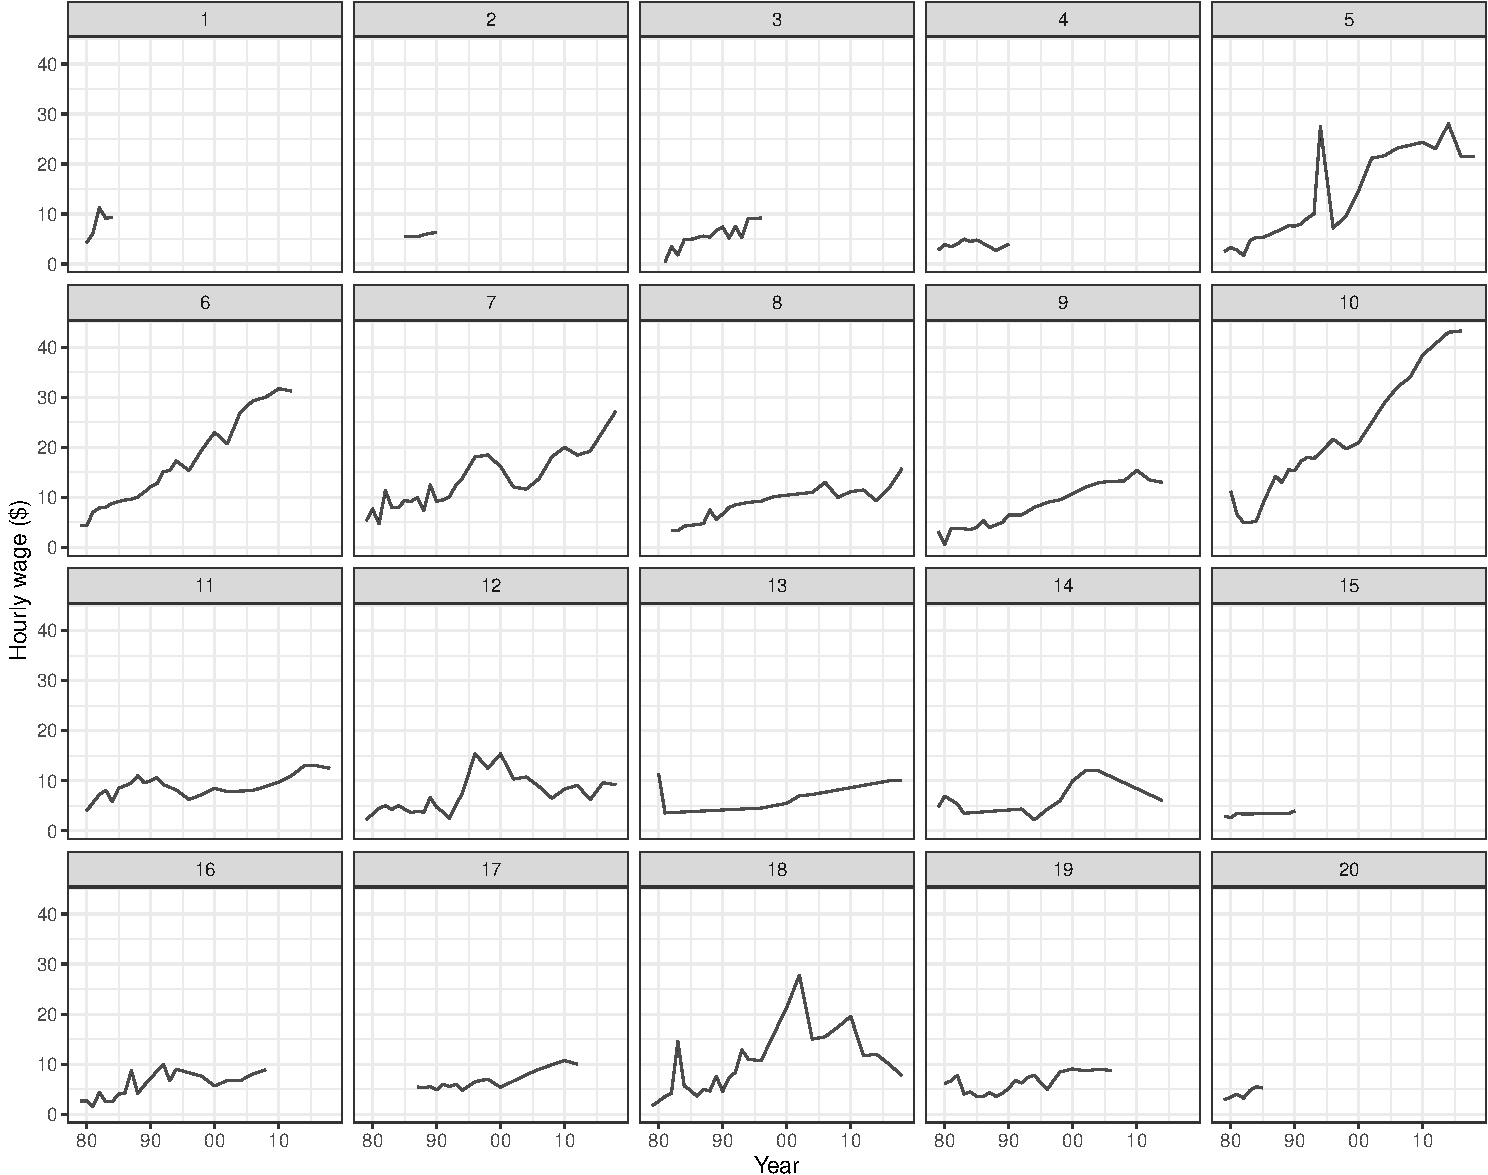
\includegraphics[width=1\linewidth]{figures/sample-plot-1}

}

\caption{Longitudinal profiles of wages for a random sample of 20 individuals in the refreshed data. Most, but not all, individuals here experienced increasing wages over time, and several have experienced considerable fluctuation in wages. Some individuals are only measured for a short period.}\label{fig:sample-plot}
\end{figure}

We randomly take 20 samples from the data and plot them, as shown in Figure \ref{fig:sample-plot}. It shows that these respondents have a lot of variability in wages, for example, the IDs in panel numbers 5, 7, and 11. The plot also implies that the samples have a different pattern of mean hourly wages. Some have had flat wages for years but had a sudden increase in one particular year, then it gone down again, while the others experienced an upsurge in their wage, for instance, the IDs in panel 9.
However, when checking the summary plots (Figure \ref{fig:feature-plot}), we found that some observations had exceptionally high wages. Some of them, for example respondents in Figure \ref {fig:feature-plot} C had experienced unusual wages only in certain year.

\begin{figure}

{\centering 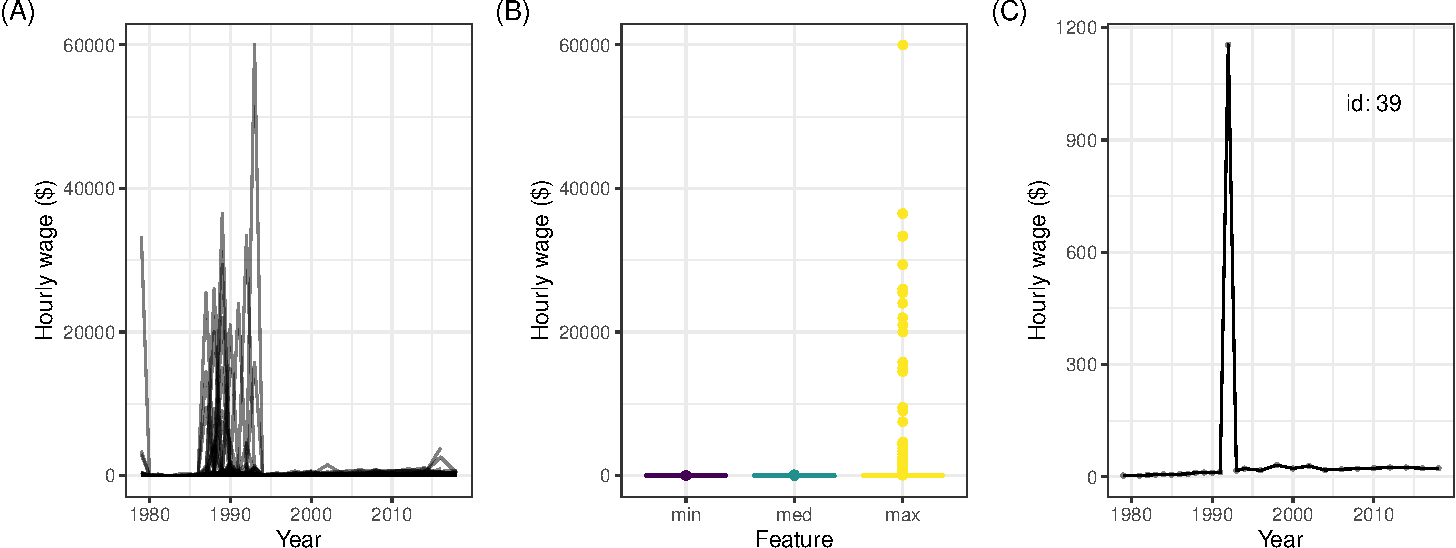
\includegraphics[width=1\linewidth]{figures/feature-plot-1}

}

\caption{Summary plots to check the cleaned data reveal more cleaning is necessary: longitudinal profiles of wages for all individuals 1979-2018 (A), boxplots of minimum, median, and maximum wages of each individual (B), and one individual (id=39) with an unusual wage relative to their years of data (C). Some values of hourly wages are unbelievable, and some individuals have extemely unusual wages in some years.}\label{fig:feature-plot}
\end{figure}

The anomalies are also found in the total hours of work, where some observations reported as having worked for 420 hours a week in total.
According to Pergamit et al. (2001), one of the flaws of the NLSY79 employment data is that the NLSY79 collects the information of the working hours since the last interview. Thus, it might be challenging for the respondents to track the within-job hours' changes between survey years, especially for the respondents with fluctuating working hours or seasonal jobs. It even has been more challenging since 1994, after which respondents were only surveyed every other year and thus had to recall two full years' job history. This shortcoming might also contribute to the fluctuation of one's wages data.

\hypertarget{censor}{%
\subsubsection{Replacing extreme values}\label{censor}}

As part of the IDA, which is the model formulation, we build a robust linear regression model to treat the extreme values in the data. Robust linear regression yields an estimation robust to the influence of noise or contamination (Koller 2016). It also aims to detect the contamination by weighting each observation based on how ``well-behaved'' they are, known as robustness weight. An observation with a lower robustness weight would be suggested as an outlier (Koller 2016).

Since we work with longitudinal data, we build the model for each ID instead of the overall data. The robust mixed model could be the best model to be employed in this case. However, this method is too computationally and memory expensive, especially for a large data set, like the NLSY79 data. Therefore, the model for each ID is built utilizing the \texttt{nest} and \texttt{map} function from \texttt{tidyr} (Wickham 2020) and \texttt{purrr} (Henry and Wickham 2020), respectively. The full code for this is shown at \url{CENSORED/articles/input-to-valid-data.html} but also described in detail next.

We build the model using the \texttt{rlm} function from \texttt{MASS} package (Venables and Ripley 2002). We set the \texttt{mean\_hourly\_wage} and \texttt{year} as the dependent and predictor, respectively. Furthermore, we use M-Estimation with Huber weighting, where the observation with a slight residual gets a weight of 1, while the larger the residual, the smaller the weight (less than 1) (UCLA: Statistical Consulting Group 2021). However, the challenging part of detecting the anomaly using the robustness weight is determining the weight threshold in which the observations are considered outliers. Moreover, it should be noted that not all the outliers are due to an error. Instead, it might be that one had reasonably increasing or decreasing wages in a particular period.

To minimize the risk of mistakenly identifying an outlier as an ``erroneous outlier'', we simulate some thresholds and study how they affect the data. We find that 0.12 is the most reasonable value to be the threshold to minimize that drawback's risk because it still captures the sensible spikes in the data. In other words, we keep maintaining the natural variability of the wages while minimizing anomalies because of the error in the data recording. After deciding the threshold, we impute the observations whose weights are less than 0.12 with the models' predicted value. We then flag those observations in a new variable called \texttt{is\_pred}.

Figure \ref{fig:compare-plot} shows the mean hourly wage before and after the extreme values are replaced. It implies that the fluctuation can still be observed in the data after the treatment. However, the large spikes, which are considered ``erroneous outliers'', are already eliminated from the data. Hence, the model produces a data set with a more reasonable degree of fluctuation.

\begin{figure}

{\centering 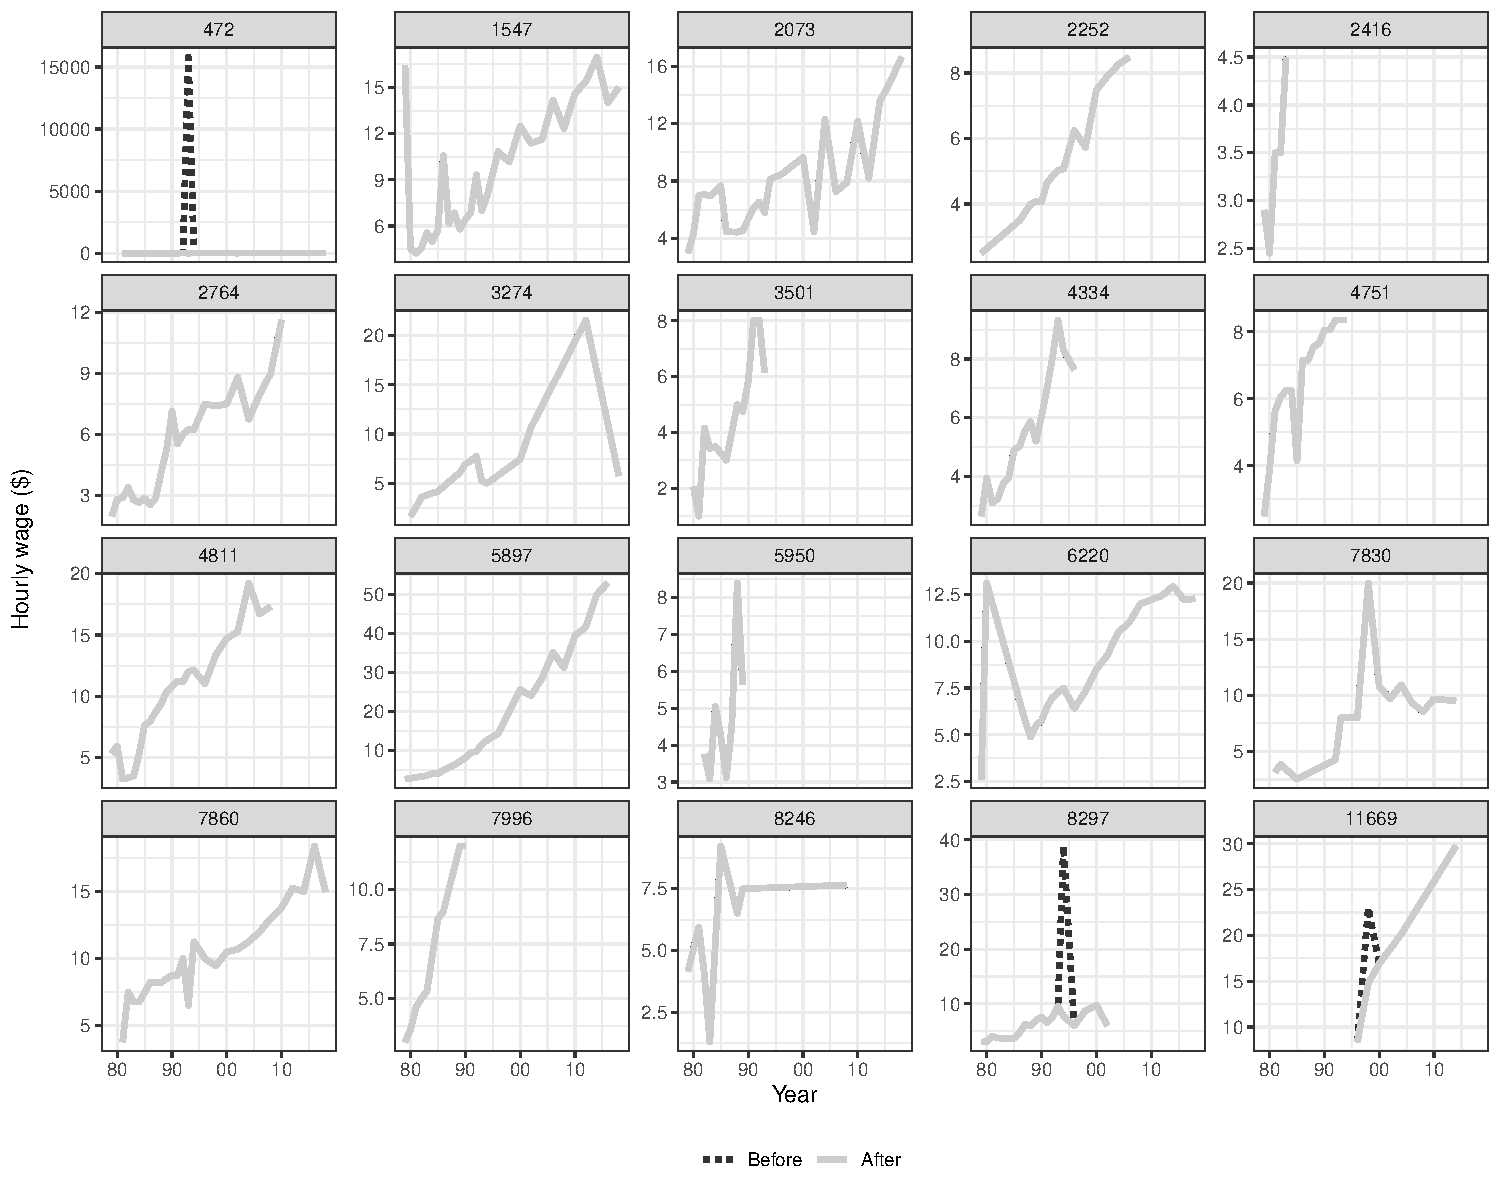
\includegraphics[width=0.9\linewidth]{figures/compare-plot-1}

}

\caption{Comparison between the original (black dots) and the corrected (solid grey) mean hourly wage for a sample of individuals. A robust linear model prediction was used to correct mean hourly wages value. We can see that some extreme spikes, corresponding to implausible wages, have been replaced with values more similar to wages in neighboring years, but otherwise the profiles are not changed. Some spikes might remain when wage vaues are plausible.}\label{fig:compare-plot}
\end{figure}

Further, Figure \ref{fig:fixed-feature-plot} A shows that after eliminating the extreme values, the highest value has decreased to be around \$350. The spikes are still observed but not as extreme as the original data set. In Figure \ref{fig:fixed-feature-plot} B, we plot the three features of mean hourly wages, namely the minimum, median, and maximum value.
We still can see some extreme values in maximum wages, but consider it as a natural variability of the data. In Figure \ref{fig:fixed-feature-plot} C, we can see that after imputing the extreme value in ID=39, we can see how the the wages change over the years more clearly.

\begin{figure}

{\centering 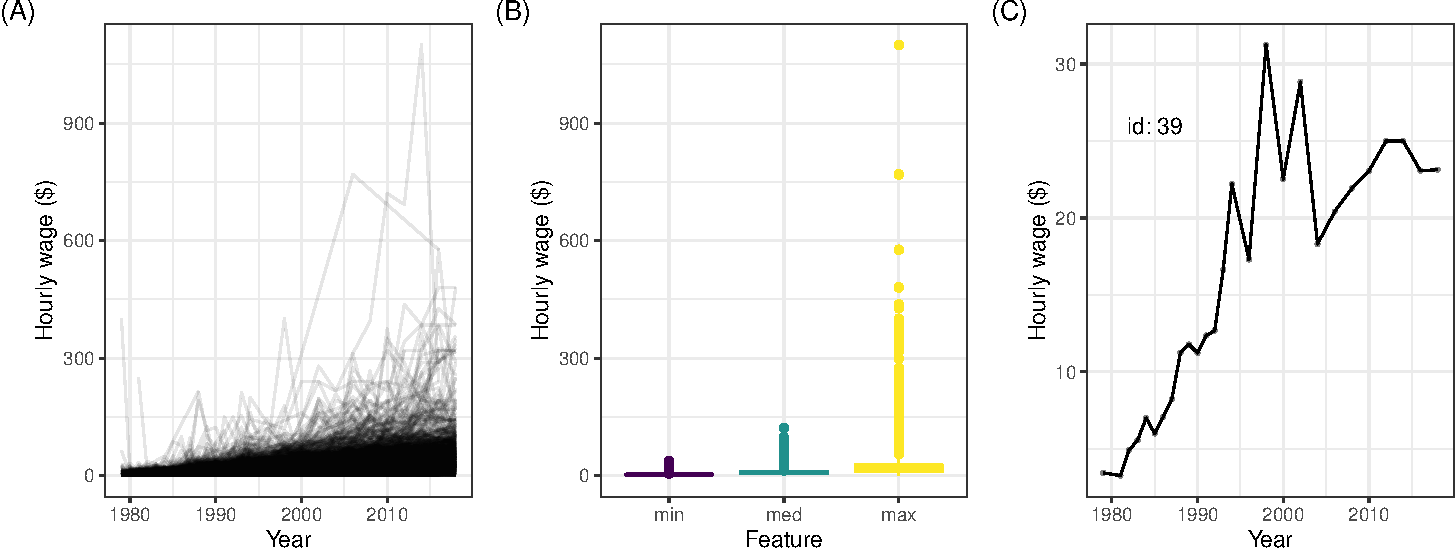
\includegraphics[width=1\linewidth]{figures/fixed-feature-plot-1}

}

\caption{Re-make of the summary plots of the fully processed data suggest that it is now in a reasonable state: longitudinal profiles of wages for all individuals 1979-2018 (A), boxplots of minimum, median, and maximum wages of each individual (B), and one individual with an unusual wage relative to their years of data (C). }\label{fig:fixed-feature-plot}
\end{figure}

Finally, we save the imputed data and set the appropriate data type for the variables.

\hypertarget{recap}{%
\subsection{Recap}\label{recap}}

Figure \ref{fig:flow-chart-blind} summarizes the steps taken to go from raw to input to valid data (van der Loo and de Jonge 2018) to create a refreshed wages data set.



\begin{figure}

<<<<<<< HEAD
{\centering \includegraphics[width=0.85\linewidth]{/Users/deeamaliah/Documents/yowie-paper/paper/figures/flowchart_blind} 
=======
{\centering \includegraphics[width=0.85\linewidth]{/Users/etan0038/Dropbox/repo/yowie-paper/paper/figures/flowchart_blind}
>>>>>>> e9174550e6e3a231aa9c7572667f6c47600e0929

}

\caption{The stages of data cleaning from the raw data to get three datasets contained in \texttt{[CENSORED]}. ``\# of individuals'' means the number of respondents included in each stage, while ``\# of observations'' means the number of rows in the data. The color represents the stage of data cleaning in statistical value chain (van der Loo and de Jonge 2021). Pink, blue, and green represent the raw, input, and valid data, respectively.}\label{fig:flow-chart-blind}
\end{figure}

\hypertarget{compare}{%
\section{Comparison of refreshed with the original data}\label{compare}}

The original set contains wages of high school dropouts (Singer and Willett 2003) from 1979 through to 1994. The refreshed data set for comparison is also wages on high school dropouts from 1979 to 2018. The original set is available in the R package \texttt{brolgar} and the refreshed data is available in the R package \texttt{[CENSORED]}.

\begin{figure}

{\centering 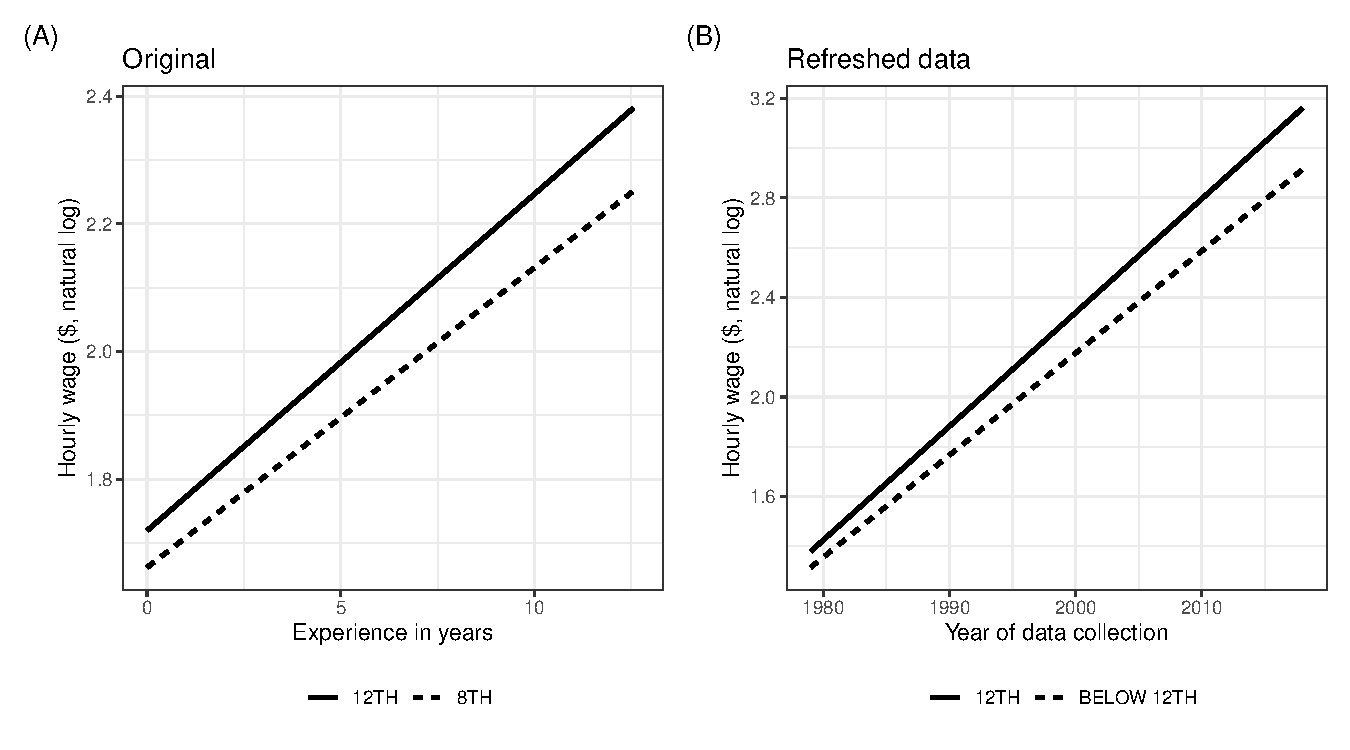
\includegraphics[width=1\linewidth]{figures/plotting-sw-do-1}

}

\caption{Comparison of original textbook example (A) with refreshed data (B). The original data was inflation-adjusted to 1990 prices and the individual's time of collection was converted to a length of experience in the workforce, which makes it difficult to precisely compare the two sets.}\label{fig:plotting-sw-do}
\end{figure}

There are two aspects of the original data that make a direct comparison difficult. Th first one is that The time variable provided is ``experience in the workforce''. It is not clear how this is calculated. One would expect that there is a record of the day the individual first started a job, and this is used to adjust the year of collection. Secondly, wages were inflation-adjusted to 1990 prices, which is not done for the refreshed data.

\textbackslash begin\{figure\}

\{\centering 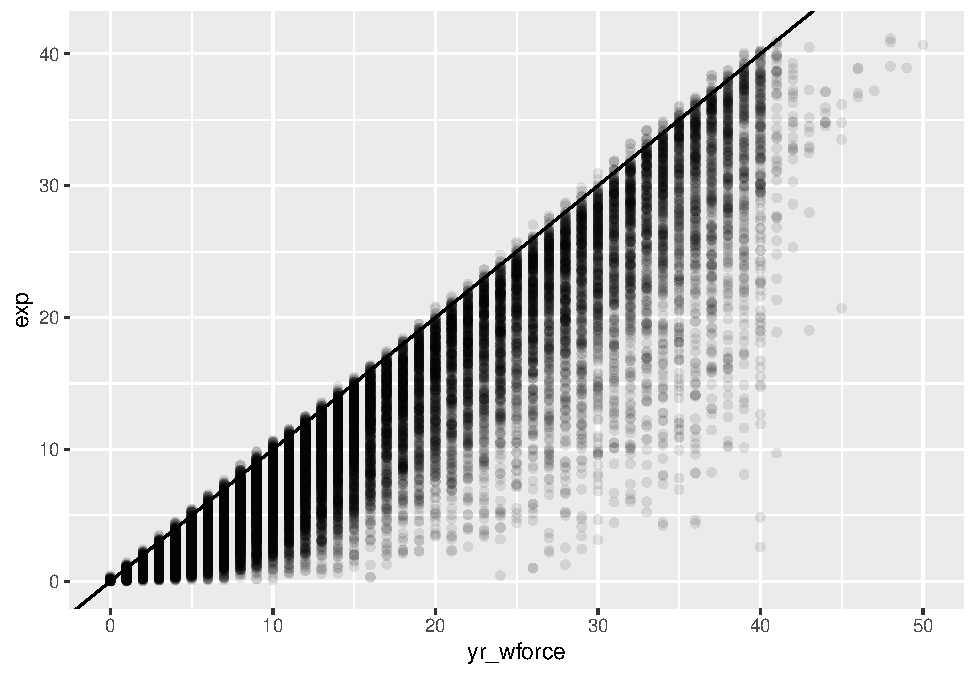
\includegraphics[width=468px]{figures/compare_xp_to_yrworkforce-1}

\}

\caption{The association between the lenght of time in the workforce (years) and the work experience. The color represents the respondents (id). Generally, the longer someone were in the workforce, the higher the work experience. However, some of the respondents have much lower working experience compared their duration in the workforce.}

(\#fig:compare\_xp\_to\_yrworkforce)
\textbackslash end\{figure\}

\begin{center}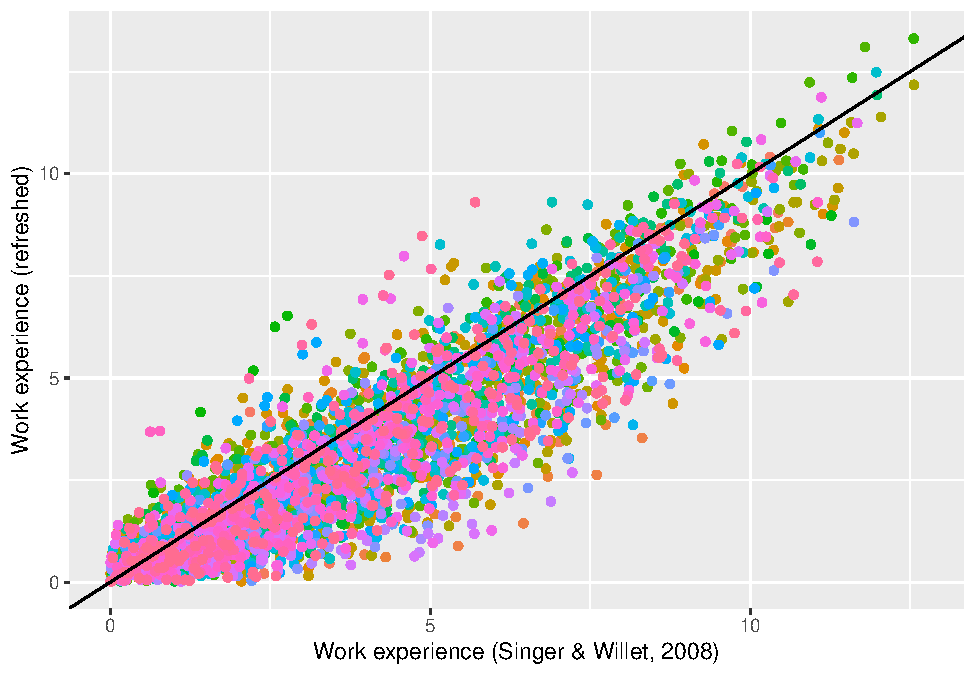
\includegraphics[width=468px]{figures/compare_xp_sw-1} \end{center}

The treatment of unlikely wages differ in the refreshed data. In the original data by Singer and Willett (2003), wages greater than \$75 are set to be missing. However, in recent context, this value is too low to be set as the maximum threshold. We opted to use the weights from a robust linear regression to determine what should be set as missing value as described in Section \ref{censor}.

Figure \ref{fig:plotting-sw-do} shows a comparison of the two sets. (A direct ID matching is not possible.) There are 888 individuals in the original and 1,188 individuals in the refreshed data. This suggests some individuals were removed in the original data.
In addition, in the original set the racial breakdown was 246 Black, 204 Hispanic and 438 White participants, while in the refreshed data there are 346 Black, 219 Hispanic, and 623 White participants, so the proportions have not been exactly reproduced. On education, in the refreshed data there are very few individuals with less than a 12th grade education, which is different from the original. In the original data there were 366 individuals with up to 8th grade and 522 9th-12th grade, as compared to 967 with 12th grade in the refreshed data.

\hypertarget{summary}{%
\section{Summary}\label{summary}}

This paper has described the stages to take a particular open data set and make it a textbook data set, ready for the classroom or research. In the first stage, we showed the steps performed to get the data from the NLSY79 database. The data format needed conversion to tidy format, and this was described. After that, an initial data analysis was conducted to investigate and screen the quality of the data. We found and fixed the anomalous observations in wages using a robust linear regression model. Finally a comparison is made between the original and refreshed data sets.

The data cleaning process is documented and the code has been made available. These provide the opportunity to again refresh the textbook data as updated data is published in the NLSY79 database.
Determining the appropriate robustness weight to threshold the anomalous observations is documented, and a \texttt{shiny} (Chang et al. 2020) app is provided to assist.
The current subset is made available in a new R package, called \texttt{[CENSORED]}.

Various difficulties were encountered in trying to refresh the data, which include:

\begin{itemize}
\tightlist
\item
  determining which records should be downloaded from the database.
\item
  there are many errors in the data, e.g.~hourly wages greater than \$30,000 per hour.
\item
  there is no explicit variable in the database recording high school dropout, which means we needed to compare date of 12th grade with the individual's age.
\item
  calculating experience in the workforce would require knowing the time of first job within the first year the individual was recorded.
\end{itemize}

Ultimately, the refreshed data is reasonably similar to the original, but unsatisfactorily far from it. The last step required would be to inflation-adjust wages, but this is better to do with each wave of new data added, so that it is relative to the last date in the data.

Some readers may disagree with our decisions made to produce the refreshed textbook data and may have better insight than us in producing a more appropriate textbook data. We do not assert that we have produced the best textbook data, but rather we describe our journey to provide a reasonable textbook data set. All code and documentation are provided for transparency, and future updates of the \texttt{[CENSORED]} package may contain additional variables, or filters of the full set, if it is deemed important.

Finally, for the data providers we recommend that a validation system with clear rules is added on data entry, and that alternative output formats, such as a tidy format would help users make better use of the resource. The problem with many of the wages records is that there are implausible values, or confusion on how to record wages for multiple jobs. These values can be validated with simple checks at data entry. Providing an open data resource also is accompanied with the responsibility that the data, especially data that is as valuable as this, is reliable. Users need to be able to trust the data.

\hypertarget{acknowledgements}{%
\section{Acknowledgements}\label{acknowledgements}}

We would like to thank Aarathy Babu for the insight and discussion during the writing of this paper.

The entire analysis is conducted using \texttt{R} (R Core Team 2020) in RStudio IDE using these packages: \texttt{tidyverse} (Wickham, Averick, et al. 2019), \texttt{ggplot2} (Wickham 2016), \texttt{dplyr} (Wickham, François, et al. 2020), \texttt{readr} (Wickham and Hester 2020), \texttt{tidyr} (Wickham 2020), \texttt{stringr} (Wickham 2019), \texttt{purrr} (Henry and Wickham 2020), \texttt{brolgar} (Tierney, Cook, and Prvan 2020), \texttt{patchwork} (Pedersen 2020), \texttt{kableExtra} (Zhu 2019), \texttt{MASS} (Venables and Ripley 2002), \texttt{janitor} (Firke 2020), and \texttt{tsibble} (Wang, Cook, and Hyndman 2020). The paper was generated using \texttt{knitr} (Xie 2014) and \texttt{rmarkdown} (Xie, Dervieux, and Riederer 2020).

\hypertarget{supplementary-materials}{%
\section{Supplementary Materials}\label{supplementary-materials}}

\begin{itemize}
\item
  \textbf{Codes}: R script to reproduce data tidying and cleaning is available in this \href{CENSORED/articles/process-data.html}{page}.
\item
  \textbf{R Package}:\texttt{[CENSORED]} is a data container R package that contains 3 datasets, namely the high school mean hourly wage data, high school dropouts mean hourly wage data, and demographic data of the NLSY79 cohort. This package can be accessed \href{CENSORED}{here}.
\item
  \textbf{shiny app}: An interactive \texttt{shiny} web app to visualise the effect of selecting different weight threshold for substituting the wages data to its predicted value from a fit of the robust linear regression model. This app can be accessed \href{CENSORED}{here} with the source code provided \href{CENSORED/tree/master/app}{here}.
\end{itemize}

\hypertarget{data-availability-statement}{%
\section{Data Availability Statement}\label{data-availability-statement}}

The authors confirm that the data supporting the findings of this study are available within the supplementary materials.

\hypertarget{references}{%
\section*{References}\label{references}}
\addcontentsline{toc}{section}{References}

\hypertarget{refs}{}
\leavevmode\hypertarget{ref-iris-data}{}%
Andereson, Edgar. 1935. ``The Irises of the Gaspe Peninsula.'' \emph{Bulletin of the American Iris Society} 59: 2--5.

\leavevmode\hypertarget{ref-nlsy79}{}%
Bureau of Labor Statistics, U.S. Department of Labor. 2021. ``National Longitudinal Survey of Youth 1979 Cohort, 1979-2016 (Rounds 1-28).'' Produced and distributed by the Center for Human Resource Research (CHRR), The Ohio State University. Columbus, OH.

\leavevmode\hypertarget{ref-shiny}{}%
Chang, Winston, Joe Cheng, JJ Allaire, Yihui Xie, and Jonathan McPherson. 2020. \emph{shiny: Web Application Framework for R}. \url{https://CRAN.R-project.org/package=shiny}.

\leavevmode\hypertarget{ref-Chatfield1985TIEo}{}%
Chatfield, C. 1985. ``The Initial Examination of Data.'' \emph{Journal of the Royal Statistical Society. Series A. General} 148 (3): 214--53.

\leavevmode\hypertarget{ref-eliznlsy}{}%
Cooksey, Elizabeth C. 2017. ``Using the National Longitudinal Surveys of Youth (Nlsy) to Conduct Life Course Analyses.'' In \emph{Handbook of Life Course Health Development}, edited by Richard M. Lerner Neal Halfon Christoper B. Forrest, 561--77. Cham: Springer. \url{https://doi.org/https://doi.org/10.1007/978-3-319-47143-3_23}.

\leavevmode\hypertarget{ref-DasuTamraparni2003Edma}{}%
Dasu, Tamraparni, and Theodore Johnson. 2003. \emph{Exploratory Data Mining and Data Cleaning}. Wiley Series in Probability and Statistics. Hoboken: WILEY.

\leavevmode\hypertarget{ref-janitor}{}%
Firke, Sam. 2020. \emph{janitor: Simple Tools for Examining and Cleaning Dirty Data}. \url{https://CRAN.R-project.org/package=janitor}.

\leavevmode\hypertarget{ref-racismnotrace}{}%
Fullilove, M. T. 1998. ``Comment: Abandoning ``Race" as a Variable in Public Health Research--an Idea Whose Time Has Come.'' \emph{American Journal of Public Health} 88 (9): 1297--8.

\leavevmode\hypertarget{ref-grimshaw}{}%
Grimshaw, Scott D. 2015. ``A Framework for Infusing Authentic Data Experiences Within Statistics Courses.'' \emph{The American Statistician} 69 (4): 307--14. \url{https://doi.org/10.1080/00031305.2015.1081106}.

\leavevmode\hypertarget{ref-purrr}{}%
Henry, Lionel, and Hadley Wickham. 2020. \emph{purrr: Functional Programming Tools}. \url{https://CRAN.R-project.org/package=purrr}.

\leavevmode\hypertarget{ref-penguins-data}{}%
Horst, Allison Marie, Alison Presmanes Hill, and Kristen B Gorman. 2020. \emph{Palmerpenguins: Palmer Archipelago (Antarctica) Penguin Data}. \url{https://doi.org/10.5281/zenodo.3960218}.

\leavevmode\hypertarget{ref-HuebnerMariannePhD2016Asat}{}%
Huebner, Marianne, Werner Vach, and Saskia le Cessie. 2016. ``A Systematic Approach to Initial Data Analysis Is Good Research Practice.'' \emph{The Journal of Thoracic and Cardiovascular Surgery} 151 (1): 25--27.

\leavevmode\hypertarget{ref-ilk2004}{}%
Ilk, Ozlem. 2004. ``Exploratory Multivariate Longitudinal Data Analysis and Models for Multivariate Longitudinal Binary Data.'' PhD thesis, Iowa State University. \url{https://doi.org/10.31274/rtd-180813-11012}.

\leavevmode\hypertarget{ref-tamedata}{}%
Kim, A. Y, C. Ismay, and J. Chunn. 2018. ``The Fivethirtyeight R Package: ``Tame Data" Principles for Introductory Statistics and Data Science Courses.'' \emph{Technology Innovations in Statistics Education} 11 (1). \url{https://doi.org/10.5070/T511103589}.

\leavevmode\hypertarget{ref-KollerManuel2016rARP}{}%
Koller, Manuel. 2016. ``robustlmm: An R Package for Robust Estimation of Linear Mixed-Effects Models.'' \emph{Journal of Statistical Software} 75 (6): 1--24.

\leavevmode\hypertarget{ref-opendata}{}%
Open Knowledge Foundation. 2021. ``Open Definition. Defining Open in Open Data, Open Content, and Open Knowledge.'' 2021. \url{http://opendefinition.org/od/2.1/en/}.

\leavevmode\hypertarget{ref-patchwork}{}%
Pedersen, Thomas Lin. 2020. \emph{patchwork: The Composer of Plots}. \url{https://CRAN.R-project.org/package=patchwork}.

\leavevmode\hypertarget{ref-MichaelRPergamit2001DWTN}{}%
Pergamit, Michael R., Charles R. Pierret, Donna S. Rothstein, and Jonathan R. Veum. 2001. ``Data Watch: The National Longitudinal Surveys.'' \emph{The Journal of Economic Perspectives} 15 (2): 239--53.

\leavevmode\hypertarget{ref-R}{}%
R Core Team. 2020. \emph{R: A Language and Environment for Statistical Computing}. Vienna, Austria: R Foundation for Statistical Computing. \url{https://www.R-project.org/}.

\leavevmode\hypertarget{ref-SingerJudithD2003Alda}{}%
Singer, Judith D, and John B Willett. 2003. \emph{Applied Longitudinal Data Analysis: Modeling Change and Event Occurrence}. Oxford u.a: Oxford Univ. Pr.

\leavevmode\hypertarget{ref-notiris}{}%
Stodel, Megan. 2020. ``Stop Using Iris.'' \url{https://www.meganstodel.com/posts/no-to-iris/}.

\leavevmode\hypertarget{ref-brolgar}{}%
Tierney, Nicholas, Di Cook, and Tania Prvan. 2020. \emph{brolgar: BRowse Over Longitudinal data Graphically and Analytically in R}. \url{https://github.com/njtierney/brolgar}.

\leavevmode\hypertarget{ref-tukey}{}%
Tukey, John W. (John Wilder). 1977. \emph{Exploratory Data Analysis}. Addison-Wesley Series in Behavioral Science. Reading, Mass.: Addison-Wesley Pub. Co.

\leavevmode\hypertarget{ref-rlm}{}%
UCLA: Statistical Consulting Group. 2021. ``Robust Regression \textbar{} R Data Analysis Examples.'' February 2021. \url{https://stats.idre.ucla.edu/r/dae/robust-regression/}.

\leavevmode\hypertarget{ref-LooMarkvander2018Sdcw}{}%
van der Loo, Mark, and Edwin de Jonge. 2018. \emph{Statistical Data Cleaning with Applications in R}.

\leavevmode\hypertarget{ref-validate}{}%
van der Loo, Mark P. J., and Edwin de Jonge. 2021. ``Data Validation Infrastructure for R.'' \emph{Journal of Statistical Software} 97 (10): 1--31. \url{https://doi.org/10.18637/jss.v097.i10}.

\leavevmode\hypertarget{ref-mass}{}%
Venables, W. N., and B. D. Ripley. 2002. \emph{Modern Applied Statistics with S}. Fourth. New York: Springer. \url{http://www.stats.ox.ac.uk/pub/MASS4}.

\leavevmode\hypertarget{ref-tsibble}{}%
Wang, Earo, Dianne Cook, and Rob J Hyndman. 2020. ``A New Tidy Data Structure to Support Exploration and Modeling of Temporal Data.'' \emph{Journal of Computational and Graphical Statistics} 29 (3): 466--78. \url{https://doi.org/10.1080/10618600.2019.1695624}.

\leavevmode\hypertarget{ref-plyr}{}%
Wickham, Hadley. 2011. ``The Split-Apply-Combine Strategy for Data Analysis.'' \emph{Journal of Statistical Software, Articles} 40 (1): 1--29. \url{https://doi.org/10.18637/jss.v040.i01}.

\leavevmode\hypertarget{ref-WickhamHadley2014TD}{}%
---------. 2014. ``Tidy Data.'' \emph{Journal of Statistical Software} 59 (10): 1--23.

\leavevmode\hypertarget{ref-ggplot2}{}%
---------. 2016. \emph{ggplot2: Elegant Graphics for Data Analysis}. Springer-Verlag New York. \url{https://ggplot2.tidyverse.org}.

\leavevmode\hypertarget{ref-stringr}{}%
---------. 2019. \emph{stringr: Simple, Consistent Wrappers for Common String Operations}. \url{https://CRAN.R-project.org/package=stringr}.

\leavevmode\hypertarget{ref-tidyr}{}%
---------. 2020. \emph{tidyr: Tidy Messy Data}. \url{https://CRAN.R-project.org/package=tidyr}.

\leavevmode\hypertarget{ref-tidyverse}{}%
Wickham, Hadley, Mara Averick, Jennifer Bryan, Winston Chang, Lucy D'Agostino McGowan, Romain François, Garrett Grolemund, et al. 2019. ``Welcome to the tidyverse.'' \emph{Journal of Open Source Software} 4 (43): 1686. \url{https://doi.org/10.21105/joss.01686}.

\leavevmode\hypertarget{ref-dplyr}{}%
Wickham, Hadley, Romain François, Lionel Henry, and Kirill Müller. 2020. \emph{dplyr: A Grammar of Data Manipulation}. \url{https://CRAN.R-project.org/package=dplyr}.

\leavevmode\hypertarget{ref-readr}{}%
Wickham, Hadley, and Jim Hester. 2020. \emph{readr: Read Rectangular Text Data}. \url{https://CRAN.R-project.org/package=readr}.

\leavevmode\hypertarget{ref-knitr}{}%
Xie, Yihui. 2014. ``Knitr: A Comprehensive Tool for Reproducible Research in R.'' In \emph{Implementing Reproducible Computational Research}, edited by Victoria Stodden, Friedrich Leisch, and Roger D. Peng. Chapman; Hall/CRC. \url{http://www.crcpress.com/product/isbn/9781466561595}.

\leavevmode\hypertarget{ref-rmarkdown}{}%
Xie, Yihui, Christophe Dervieux, and Emily Riederer. 2020. \emph{R Markdown Cookbook}. Boca Raton, Florida: Chapman; Hall/CRC. \url{https://bookdown.org/yihui/rmarkdown-cookbook}.

\leavevmode\hypertarget{ref-kableExtra}{}%
Zhu, Hao. 2019. \emph{kableExtra: Construct Complex Table with 'kable' and Pipe Syntax}. \url{https://CRAN.R-project.org/package=kableExtra}.


\bibliographystyle{Chicago}

\end{document}
